\section{Mutation Methods}

\subsection{Scramble Mutation}

In scramble mutation two gene indexes are selected at random. A slice of the genes is created between the 2 indexes. The new slice is then randomly shuffled and is re-inserted back into the original genes between the same indexes. This process is outlined in the image below.

\begin{figure}[h!]
\vspace{-5pt}
\centering
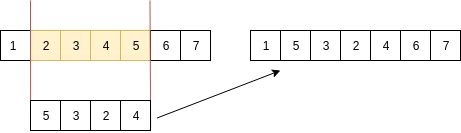
\includegraphics[width=1.0\textwidth]{images/scramble.png}
\caption{\label{fig:3col_graph}Scramble mutation}
\end{figure}

\subsection{Reciprocal Exchange Mutation}

This is a very simple mutation method. 2 Genes are selected at random and then swapped with each other.

\begin{figure}[h!]
\vspace{-5pt}
\centering
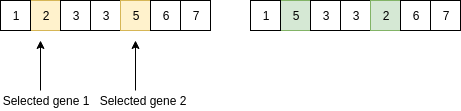
\includegraphics[width=1.0\textwidth]{images/reciprocal.png}
\caption{\label{fig:3col_graph}Reciprocal exchange mutation}
\end{figure}

In the image above, 2 and 5 are selected at random and then swapped in the resulting chromosone